\chapter{渋滞とドライブレコーダー}
% Tanimu先輩"具体的に都市の画像を用いた想定している有効活用の方法について話す.軽く"
% 俺の研究の場合どんな問題について語ればいいんだろうねよくわからん
% 多分渋滞についての問題を書けばいいのかもしれない(適当)
ここでは本研究をするにあたって、本研究が意識する問題について述べる。


\section{渋滞がもたらす影響}
渋滞中のドライバーには肉体的ストレスと精神的ストレスの両方がかかっている。
肉体的ストレスに関しては、運転中は長時間座ったままであり、狭い車内で体を伸ばすことができない、という問題が考えられる。
仮に遠出していて長時間渋滞に巻き込まれてしまうと同じ姿勢のまま運転する必要がありエコノミー症候群が発症する恐れが考えられる。
また、ドライバーの精神的ストレスに関して、東京農工大学大学院の佐藤氏\cite{alma99344256104031}は、渋滞中のドライバーの精神ストレスを以下のように述べている(\tabref{tab:stress_of_driver})。

% -------------------------------------------------------------------

\begin{table}[htbp]
  \centering
  \begin{scriptsize}
\begin{tabular}{c}
  \toprule
  精神的ストレスの種類 \\
  \midrule
  目的地に早く着きたいのに自分の意に反して進めない \\
  進もうとしているのに横入りにより邪魔される \\
  退屈する \\
  \bottomrule
\end{tabular}
\end{scriptsize}
\caption{渋滞中のドライバーの精神ストレス}
\label{tab:stress_of_driver}
\end{table}

% ---------------------------------------------------------------------


また、自動車の交通渋滞はドライバーのみに影響を与えるのではない。
東京農工大学大学院の佐藤氏によると、渋滞中の交通事故の発生率は通常の時よりも8倍高い\cite{alma99344256104031}。
特に追突事故に関しては、通常の時よりも16倍高い事故発生率となる。

交通事故の原因の多くがヒューマンエラーによるものだと考えれば、渋滞情報を事前に取得し、渋滞を回避することは、ドライバーにとっても交通安全の面においても重要な課題なことがわかる。

\newpage

\section{渋滞検知}
% 渋滞情報はどのように作られるのか
% VICSの話
現在の渋滞は主要な道路にセンサーやカメラなどを取り付けてリアルタイムに渋滞情報を検知し管理している。
渋滞情報の取得には一般財団法人道路交通情報通信システムセンター(VICS)が関わっている。
VICSではVICSセンターが国土交通省、地方自治体および都道府県警察からの渋滞情報を集めて管理している。
集められた渋滞情報はFM多重放送、電波ビーコン、光ビーコンといった道路に設置された通信機でVICS対応カーナビゲーションシステムに送信し、渋滞情報や目的地までの到着予想時刻としてドライバーが受け取っている。
また、特に高速道路における渋滞情報の取得については、道路に2km間隔でトラフィックカウンターという計測器が埋め込まれており、通過する車の台数、大型車や小型車の区別、車の速度を計測している。
トラフィックカウンターだけではなく、高速道路においては交通管理隊が常に巡回しており、渋滞を見つけると無線で交通管制センターへ連絡し、ドライバーへフィードバックしている(参照:\figref{fig:vics_system})。

\begin{figure}[htbp]
  \begin{center}
   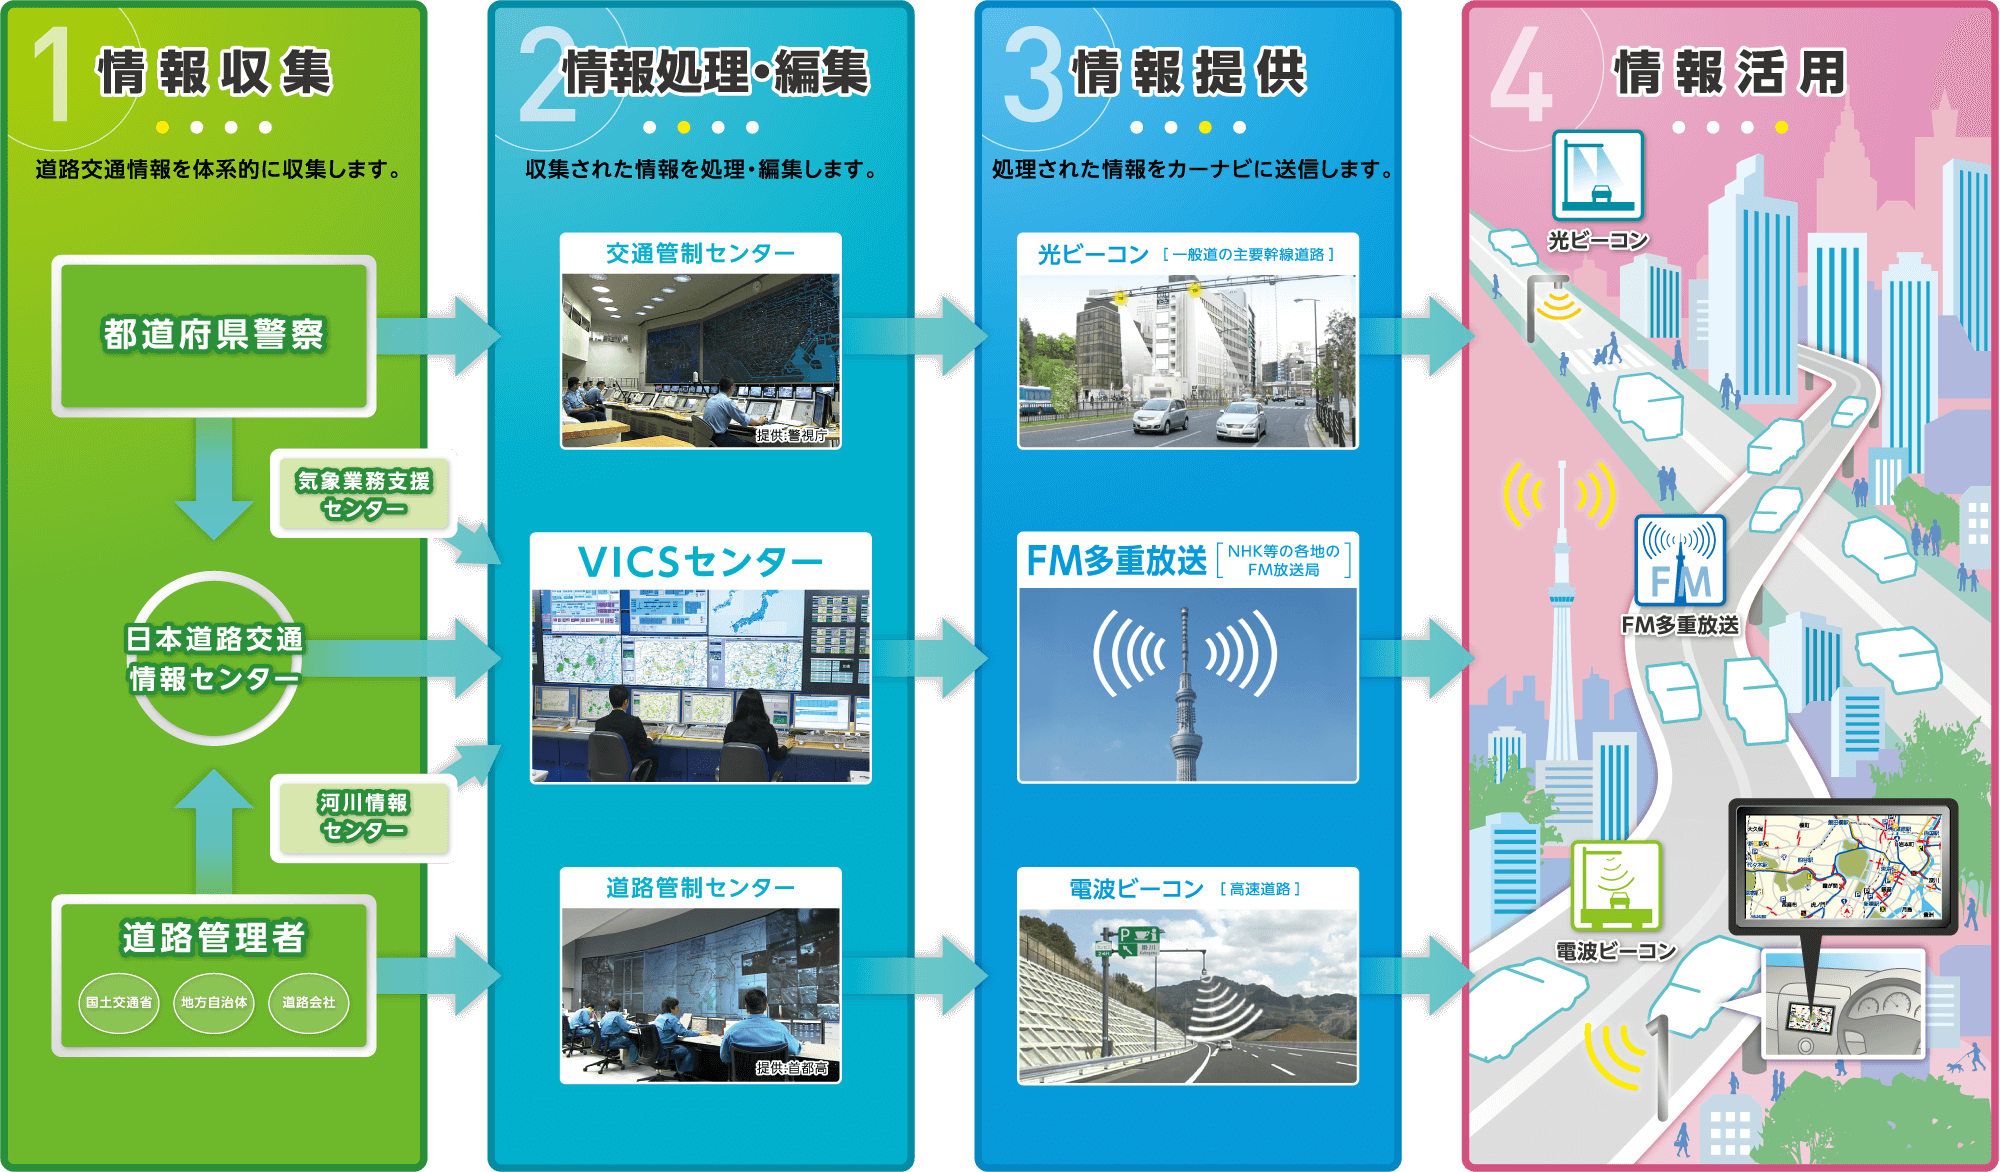
\includegraphics[width=11cm]{figs/vics.png}
  \end{center}
  \caption{VICSの仕組み(https://www.vics.or.jp/know/about/center.html)}
  \label{fig:vics_system}
\end{figure}

% それがどう不備なのか
しかし現状、渋滞情報は高速道路や国道といった主要な道路のみの情報しか得られておらず、それ以外の比較的小さい道路では渋滞情報を取得することができない問題がある。
例えば旅行シーズン中など、普段の走行量が少ない道路にて走行量が急に増えた際に、事前に渋滞情報を取得して迂回することが困難になる。
特に、1車線のような小さい道路が急な渋滞になるケースのことが多く、一度渋滞にはまってしまうと迂回ルートを取ろうとしても抜け出すことが難しくなる。

また、VICS非対応のカーナビゲーションが存在することも問題の一つである。
日本は世界的な自動車生産量を誇り、日本で走っている自動車はほとんどが国産車である。
しかし、2019年度の統計によると、日本市場における輸入車のシェアは6\%となっており、輸入車に載っている人口は一定数いることがわかる。
輸入車に乗っている人はVICS対応のカーナビゲーションを購入する必要がある。
また、日本で販売しているカーナビゲーションにもVICSに対応していない機種が存在する。

% プローブ情報を活用した例
\subsection{プローブ情報}
2020年よりVICSは渋滞ゼロ社会を目指すためにプローブ情報を利用したサービスの実証実験を行なっている(参照:\figref{fig:probe})。
プローブ情報とは、車一台一台の位置、速度、通過時刻等の等の走行軌跡データーを指す。
プローブ情報を活用することでこれまでトラフィックカウンターがなかった場所でも渋滞情報を取得することを目指し、実証実験を行なっている。

\begin{figure}[htbp]
  \begin{center}
   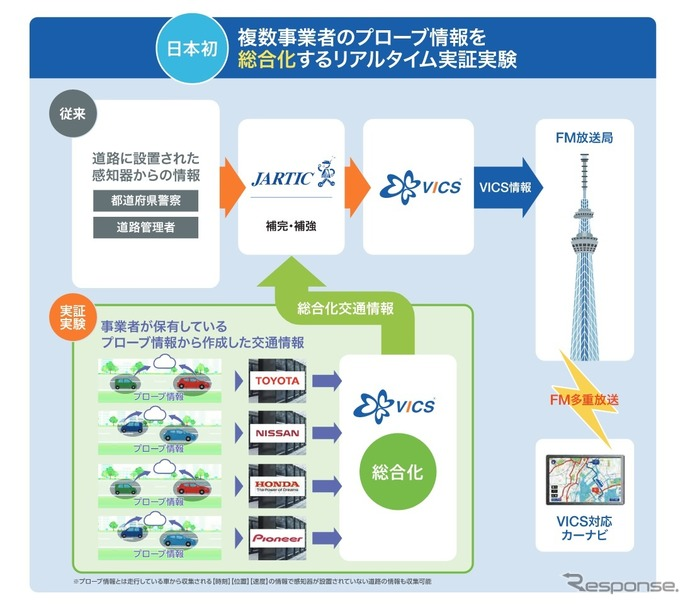
\includegraphics[width=11cm]{figs/probe.jpg}
  \end{center}
  \caption{実証実験中のプローブ情報を利用したシステム(https://response.jp/article/2020/03/05/332331.html)}
  \label{fig:probe}
\end{figure}

しかし、プローブ情報には車のセンサーを主に使っているため、ドライブレコーダーを使う等の情報はない。
センサーの情報のみを使って渋滞検知を行おうとすると、例えば低速運行しているのは渋滞に巻き込まれたからなのか、他の理由があるからなのか等の情報を得ることができない。
また、車が停止したのは渋滞のためなのか、停止信号のためなのか、あるいは駐車のためなのかといった情報もセンサーからのみでは得ることができない。
これらの情報を得るにあたって、ドライブレコーダーの使用は避けて通れないと考える。

% 渋滞に巻き込まれなくなることのメリットとか書いたほうがいいかな?
\newpage
\section{ドライブレコーダー}
% ドライブレコーダーの問題点
次に、ドライブレコーダーについて述べる。
% ドライブレコーダーの搭載率
2020年1月に国道交通省が出した統計\cite{ministryofland}によると、統計対象者のうちドライブレコーダーを実際に取り付けている割合は45.9\%という結果が出た。
つまり、統計の対象になったドライバーのうちおよそ半数がドライブレコーダーを搭載していることがわかる。
また、同統計において、ドライブレコーダーの使用目的のアンケートがあり、以下のようになっている.

% ----------------------------------------------------------------

\begin{table}[htbp]
  \centering
  \begin{scriptsize}
  \begin{tabular}{ccccccc}
  \toprule
ドライブレコーダーを & 安全運転の意識 & 自分の運転のクセなど & 交通事故の記録 & 煽り運転等  & 綺麗な風景など & その他 \\
なぜ導入するか(年代別) & を高める & を把握する & & 危険な運転への対策 & の記録 & \\ 
(複数回答可) & & & & & \\
  \midrule
全年代 & 45.5\% & 10.2\% & {\bf89.8\%} & {\bf71.7\%} & 7.7\% & 5.2\% \\
20代 & 50.0\% & 10,0\% & {\bf90.0\%} & {\bf63.3\%} & 16.7\% & 6.7\% \\
30代 & 38.9\% & 13.0\% & {\bf83.3\%} & {\bf74.1\%} & 7.4\% & 13.0\% \\
40代 & 46.1\% & 6.7\% & {\bf92.1\%} & {\bf76.4\%} & 11.2\% & 4.5\% \\
50代 & 47.4\% & 5.3\% & {\bf89.5\%} & {\bf59.2\%} & 5.3\% & 5.9\% \\
60代 & 42.1\% & 12.3\% & {\bf93.0\%} & {\bf78.9\%} & 3.5\% & 1.8\% \\
70代以上 & 57.9\% & 31.6\% & {\bf89.5\%} & {\bf84.2\%} & N/A & N/A \\
  \bottomrule
  \end{tabular}
  $\scriptstyle \mbox{出典:「自動車用の映像記録型ドライブレコーダー装置について」(国土交通省)}\atop \scriptstyle \mbox{(https://www.mlit.go.jp/monitor/R1-kadai01/24.pdf)}$
\end{scriptsize}
  \caption{ドライブレコーダー導入の目的(年代別)}
  \label{tab:recoder_static_age}
\end{table}

\begin{table}[htbp]
  \centering
  \begin{scriptsize}
  \begin{tabular}{ccccccc}
  \toprule
ドライブレコーダーを & 安全運転の意識 & 自分の運転のクセなど & 交通事故の記録 & 煽り運転等  & 綺麗な風景など & その他 \\
なぜ導入するか(地域別) & を高める & を把握する & & 危険な運転への対策 & の記録 & \\ 
(複数回答可) & & & & & \\
  \midrule
北海道 & 43.5\% & 17.4\% & {\bf91.3\%} & {\bf87.0\%} & 4.3\% & 4.3\% \\
東北 & 51.9\% & 11,1\% & {\bf85.2\%} & {\bf74.1\%} & 7.4\% & 3.7\% \\
関東 & 44.4\% & 12.7\% & {\bf82.5\%} & {\bf66.7\%} & 7.9\% & 7.9\% \\
北陸 & 63.0\% & 22.2\% & {\bf85.2\%} & {\bf74.1\%} & 7.4\% & 3.7\% \\
中部 & 36.4\% & 9.1\% & {\bf93.2\%} & {\bf77.3\%} & 9.1\% & 6.8\% \\
近畿 & 38.9\% & 1.9\% & {\bf94.4\%} & {\bf70.4\%} & 3.7\% & 3.7\% \\
中国 & 39.3\% & 7.1\% & {\bf89.3\%} & {\bf57.1\%} & 17.9\% & 7.1\% \\
四国 & 56.5\% & 17.4\% & {\bf91.3\%} & {\bf69.6\%} & N/A & 4.3\% \\
九州 & 50.0\% & 2.8\% & {\bf97.2\%} & {\bf75.0\%} & 11.1\% & 2.8\% \\
  \bottomrule
  \end{tabular}
  $\scriptstyle \mbox{出典:「自動車用の映像記録型ドライブレコーダー装置について」(国土交通省)}\atop \scriptstyle \mbox{(https://www.mlit.go.jp/monitor/R1-kadai01/24.pdf)}$
\end{scriptsize}
  \caption{ドライブレコーダー導入の目的(地域別)}
  \label{tab:recoder_static_block}
\end{table}

% -------------------------------------------------------

表から分かる通り、どの年代およびどの地域でも、ドライブレコーダーを取り付ける目的としては「交通事故の記録」が最も高く、次いで「煽り運転等危険な運転への対策」、「安全運転の意識」が高くなっている。
また、同統計ではドライブレコーダーの活用状況についての統計があり、\figref{fig:use_recoder}と\figref{fig:use_recorder2}に結果を示す。

また、ドライブレコーダーを実際にどのように活用したかについてのアンケート結果があり、\tabref{tab:howto_use_rec}に結果を示す。
以上のことからわかることは、統計に参加したドライバーのうち約半数がドライブレコーダーを取り付けて入るものの、実際にドライブレコーダーの映像を活用できているのは全体の2割ほどであるということである。

%----------------------------------

\begin{figure}[htbp]
  \begin{center}
   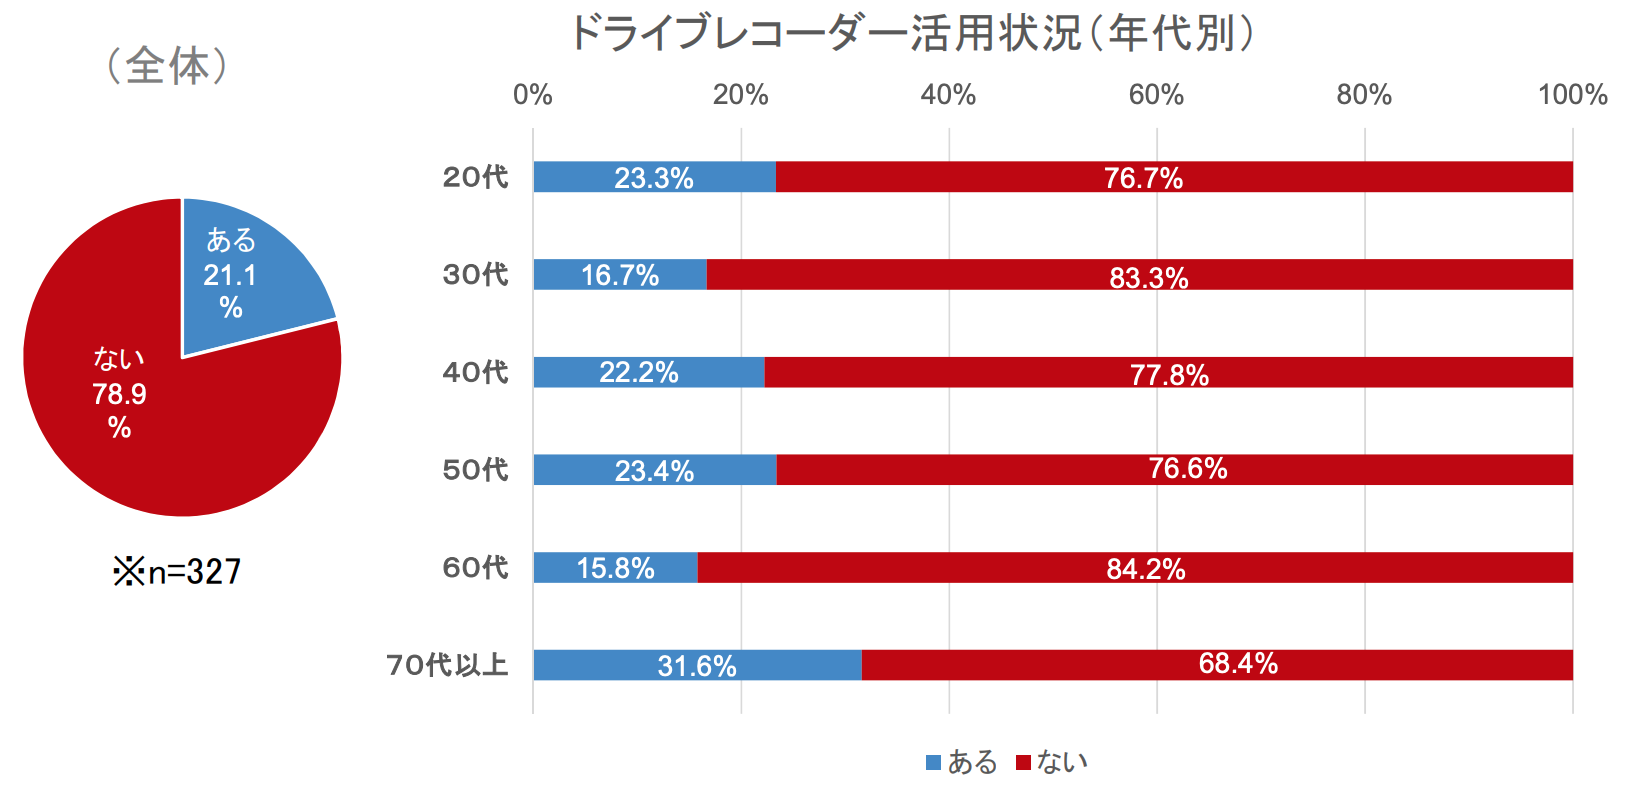
\includegraphics[width=12cm]{figs/use_driverecoder1.png}
   $\scriptstyle \mbox{出典:「自動車用の映像記録型ドライブレコーダー装置について」(国土交通省)}\atop \scriptstyle \mbox{(https://www.mlit.go.jp/monitor/R1-kadai01/24.pdf)}$
  \end{center}
  \caption{ドライブレコーダーの記録を活用したことがあるかについてのアンケート結果(年代別)\cite{ministryofland}}
  \label{fig:use_recorder}
\end{figure}

\begin{figure}[htbp]
  \begin{center}
   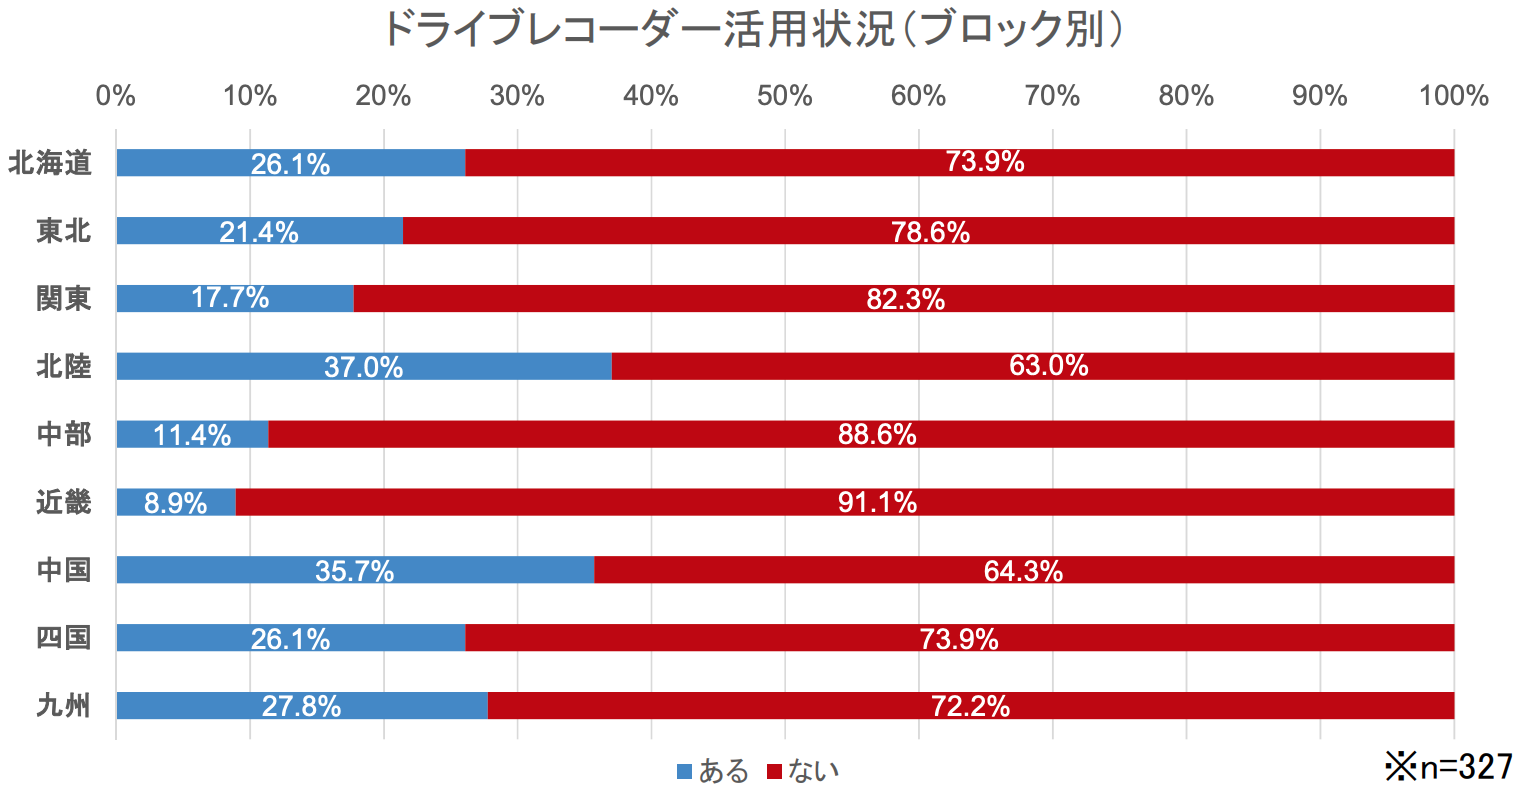
\includegraphics[width=12cm]{figs/use_driverecorder2.png}
   $\scriptstyle \mbox{出典:「自動車用の映像記録型ドライブレコーダー装置について」(国土交通省)}\atop \scriptstyle \mbox{(https://www.mlit.go.jp/monitor/R1-kadai01/24.pdf)}$
  \end{center}
  \caption{ドライブレコーダーの記録を活用したことがあるかについてのアンケート結果(ブロック別)\cite{ministryofland}}
  \label{fig:use_recorder2}
\end{figure}

\begin{table}[htbp]
  \centering
  \begin{scriptsize}
\begin{tabular}{cc}
  \toprule
状況 & ドライブレコーダーをどのように活用したか\\
  \midrule
交通事故の時 & 貰い事故の際に、自分の無過失が証明できた。\\
& 交通事故に遭遇した際に、第三者として記録を提出した。 \\
\hline
安全運転のため& 悪質な運転や犯罪の動画をもとに警察へ通報した。\\
& 事故になりかけた状況を、後日再確認した。\\
& 家族でお互いの運転を検証している。\\
& 車内での安全運転啓発に画像を利用した。 \\
& 運転中に相手車の運転を確認する。 \\
& 危険運転などの動画をSNSに投稿した。\\
\hline
その他 & 豪雨災害や隕石の落下などたまたま映っていた画像を共有した。\\
& 旅先などの景色や遭遇した野生動物などを録画した。\\
\bottomrule
\end{tabular}
$\scriptstyle \mbox{出典:「自動車用の映像記録型ドライブレコーダー装置について」(国土交通省)}\atop \scriptstyle \mbox{(https://www.mlit.go.jp/monitor/R1-kadai01/24.pdf)}$
  \end{scriptsize}
  \caption{ドライブレコーダーの活用状況}
\label{tab:howto_use_rec}
\end{table}

% ---------------------------------------------------------------------

\newpage
\section{ドライブレコーダーを使うメリット}
2.2章で述べた通り、ドライブレコーダーを設置している人口は一定数いるものの、そのほとんどがドライブレコーダーを実際に活用していないことがわかる。
本研究ではドライブレコーダーからの車間距離を推定することで渋滞を推定することを目的としているが、この車間距離の推定をすることでいずれは煽り運転の推定や警告などドライバーにとって有益な情報提供ができる研究に繋げることが可能だと考えられる。
また、車間距離を推定することができれば、安全運転を評価することも可能になる。
世界の情勢として、自動運転への移行に舵がとられているが、日本では法整備の問題等で完全な自動運転への移行は未だに時間がかかると予想されている。
ドライブレコーダーの映像から得られる情報は、ドライバーの見ている景色とほぼ同じだとすると、ドライブレコーダーを使って渋滞だけでは無く、道路標識や信号等も検出することが可能である。
それらの検出をもとに、ドライバーがきちんと道路標識に従って、一時停止等していたか、十分な車間距離を守って走行できていたか、というようなドライバーが安全運転だったか否かを評価することができる。
これは他のセンサーやGPSのデーターだけを用いる手法では難しく、ドライブレコーダーを活用する利点であると言える。
さらに、先行車の動きをトラッキング、分析することで煽り運転の検出、警告することも可能である。
